\newpage

\section{Aufgabe 1}

\subsection{Aufgabenstellung}
Beschreiben Sie mit eigenen Worten und einer Skizze, wie Browser-Cookies funktionieren!
(1 Punkt)

\subsection{Vorbereitung}
Für diese Aufgabe haben wir uns mit Browser-Cookies auseinander gesetzt.

\subsection{Durchführung}
Cookies werden verwendet, um Sitzungen auf Websites zu verwalten, virtuelle Einkaufswägen zu speichern oder Nutzerverhalten aufzuzeichnen.

\begin{figure}[H]
	\centering
	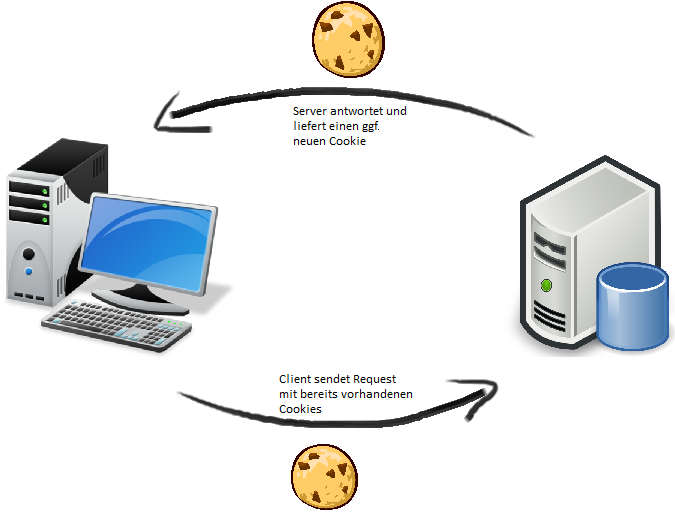
\includegraphics[width=0.6 \linewidth]{images/cookies}
	\caption{Verlauf von Cookies} \label{ordner}
\end{figure} 

Im folgenden Beispiel ist ein Request für ein Cookie zu sehen.
\begin{lstlisting}
GET /cgi/suche.py?q=cookie+aufbau HTTP/1.0
\end{lstlisting}

Dazu gehörig findet man hier die Antwort auf diesen Request. Mit Set-Cookie wird der Cookie gesetzt. Als erstes findet man im Cookie die Nutzdaten. Diese Nutzdaten können einen eigenen Namen haben. Da die Nutzdaten Zeichen enthalten können welche nicht erlaubt sind ist der Bereich Base64 verschlüsselt. Unter \textbf{expires} findet man heraus bis zu welchem Datum der Cookie gültig ist. Im Bereich \textbf{Max-Age} wird in Sekunden angegeben wie lange der Cookie mitgeschickt wird. Zu guter Letzt findet man noch den Pfad des Cookies, welcher aber nur für Suchmaschinen relevant ist.
\begin{lstlisting}
HTTP/1.0 200 OK
Set-Cookie: letzteSuche=Y29va2llIGF1ZmJhdQ==;
			expires=Tue, 29-Mar-2014 19:30:42 GMT;
			Max-Age=2592000;
			Path=/cgi/suche.py
\end{lstlisting}

\subsection{Fazit}
Cookies sind sehr simpel gehalten und für jedermann verständlich.

\section{Aufgabe 2}

\subsection{Aufgabenstellung}
Formulieren Sie mindestens fünf Kurzfragen, die in Stichworten zu beantworten sind. Die Aufgaben sollen im Stil von Klausurfragen gestellt werden. Gerne dürfen Sie eine eigene Aufgabe zur UDP Prüfsumme und der Numerierung von TCP Paketen mit Sequenz- und ACK-Nr. entwerfen und lösen. Zur Ideenfindung beachten Sie auch den Artikel zum Thema Internet Peering, der Stoff aus Vorlesung Nr. 2 wiederholt und vertieft. (2 Punkte)

\subsection{Vorbereitung}
Erneutes überfliegen der Vorlesungsinhalte und Aufgaben.

\subsection{Durchführung}

\textbf{Wie lauten die 7 Schichten des OSI Modells?}
\begin{itemize}
	\item Application Layer
	\item Presentation Layer
	\item Session Layer
	\item Transport Layer
	\item Network Layer
	\item Data Link Layer
	\item Physical Layer
\end{itemize}
\textbf{Nennen Sie 5 wichtige Protokolle der Applikations Schicht.}
\begin{itemize}
	\item HTTP
	\item FTP
	\item SMTP
	\item POP3
	\item IMAP
\end{itemize}
\textbf{Erklären Sie Multicast.}
\begin{itemize}
	\item Ein Knoten spricht mit mehreren Knoten aus der Gruppe.
	\item Kardinalität: 1:n
\end{itemize}
\textbf{Wie lauten die vier wichtigsten Funktionen von http?}
\begin{itemize}
	\item GET
	\item POST
	\item PUT
	\item DELETE
\end{itemize}
\textbf{Was ist der wichtigste Unterschied zwischen TCP und UDP?}
\begin{itemize}
	\item Im Gegensatz zu TCP ist UDP ungerichtet.
\end{itemize}

\subsection{Fazit}
Alle Fragen sind im Stil einer Klausur.

\section{Aufgabe 3}

\subsection{Aufgabenstellung}
Entwickeln Sie eine kurze Programmieraufgabe (Frage und Lösung dazu). Diese Aufgabe soll einen Teilbereich Ihrer Wahl aus dem bisher behandelten Vorlesungsstoff abdecken. (2 Punkte)

\subsection{Vorbereitung}
Für diese Aufgabe muss man sich mit den bisher behandelten Vorlesungsstoff auseinandersetzen. 

\subsection{Durchführung}

\subsubsection{Frage}
Sie haben ein RESTful API die unter folgender URL zu erreichen ist \textit{http://restapi.de}, über diese API möchten sie sich die aktuelle Uhrzeit beschaffen, diese gibt sie einfach als Zeichenkette zurück, nicht als JSON und auch nicht als XML. Wie könnte diese Anfrage aussehen unter der Verwendung von Java?

\subsubsection{Antwort}
\begin{lstlisting}
try {
	URL u = new URL('http://restapi.de');
	HttpURLConnection conn = (HttpURLConnection) u.openConnection();
	conn.setRequestMethod("GET");
	BufferedReader reader = new BufferedReader(new InputStreamReader(conn.getInputStream()));
	String output;
	while ((output = reader.readLine()) != null) {
		return output;
	}
} catch (Exception e) {
	e.printStackTrace();
}
\end{lstlisting}

\subsection{Fazit}
Die Aufgabe gab keine Probleme und sie war leicht zu lösen.

\section{Aufgabe 4}

\subsection{Aufgabenstellung}
In der Vorlesung Nr. 4 (RMI und REST) wurden mögliche Anforderungen an Middlewaretechnologien
genannt. Diese finden Sie in der Bewertung zum Thema RMI (Folien 21
bis 23). Fuhren Sie die dortige Anforderungsanalyse für REST durch. (3 Punkte) 

\subsection{Vorbereitung}
Vertraut machen mit der oben genannten Vorlesung.

\subsection{Durchführung}
\textbf{REST Performance}

\section{Aufgabe 5} 

\subsection{Aufgabenstellung}
Gegeben ist folgender Screenshot aus der Windows Systemsteuerung. Erklären Sie die Einstellungen. Zeichnen Sie das Diagramm eines kleinen Firmennetzwerkes, in dem mehrere Rechner, ein Router und ein Drucker verbunden sind (analog zu Folie 55 in Vorlesung 5). Der Screenshot zeigt die Konfiguration eines Rechners in diesem Netz. Welchen Weg nehmen Pakete, die von einem Rechner zum Drucker gesendet werden? Welchen Weg nehmen Pakete, die in das Internet geleitet werden sollen? (2 Punkte)

\subsection{Vorbereitung}
Für diese Aufgabe muss man sich mit der neusten Vorlesung auseinandersetzen oder selbst recherchieren.

\subsection{Durchführung}
Die Verbindung vom Rechner mit dem Drucker, kommt über den Router zustande, er verbindet die beiden. Der Rechner in unserem Beispiel hat eine fest IP-Adresse und wir gehen in unserem Fall davon aus das der Router eine IP-Adresse für den Drucker bereitstellt, über DHCP. Jetzt stellt der Computer eine Verbindung auf mit dem Drucker, meistens über Freigabename, der Router kennt diesen, teilt diesen mit dem Computer verbindet die beiden.\\\\Die Verbindung zwischen dem Computer und Internet ist da ziemlich unterschiedlich, der Rechner ruft z.B. eine Webseite auf, kennt dort nur den FQDN und gibt diesen an den Router weiter. Dieser gibt diesen FQDN an einen, an ihm eingestellten, DNS-Server weiter, welcher ihm eine IP-Adresse zurückliefert und diese Daten die er von dieser IP-Adresse bekommt übers HTTP-Protokoll gibt er an den Rechner zurück. Als Grafik siehe \autoref{internet}.

\begin{figure}[H]
	\centering
	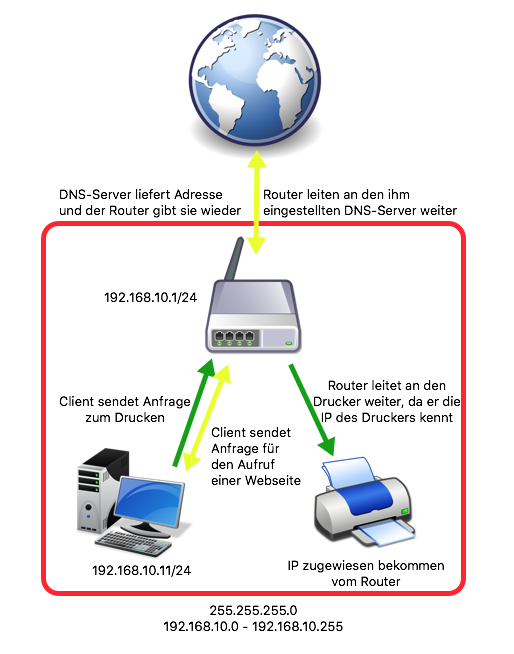
\includegraphics[width=0.6 \linewidth]{images/internet}
	\caption{Verbindungen} \label{internet}
\end{figure}  

\subsection{Fazit}
Diese Aufgabe war umfangreicher als die anderen Aufgaben, war aber auch etwas schwieriger.


